\chapter{完整性与安全性}

\begin{introduction}[期末考试提纲]
    \item 完整性定义
    \item 约束级别、约束类型、约束检查、延迟约束
    \item 安全性定义
    \item 角色、权限、统计数据库安全
\end{introduction}

\section{数据完整性}

\textbf{约束的对象级别}:
\begin{itemize}
    \item 列级约束, 列值范围. e.g., \textit{sno要求是8位整数, 首位是0或1; 选课人数不能少于10人, 多于100人.}
    \item 行级约束, 同一行各列之间. e.g., \textit{飞行员的星级评定取决于其飞行里程.}
    \item 表级约束, 行间、表上、表间. e.g., \textit{在本地纳税记录超过5年才有购房资格.}
\end{itemize}

\textbf{约束类型}:
\begin{itemize}
    \item primary key;
    \item foreign key;
    \item unique;
    \item default;
    \item not null;
    \item check.
\end{itemize}

存储约束的系统表: sysconstraints.
\begin{table}[H]
    \centering
    \begin{tabular}{|l|l|l|}
        \hline
        \textbf{列名} & \textbf{数据类型} & \textbf{描述} \\ \hline
        constid & int & 约束号 \\ \hline
        id & int & 拥有该约束的表 ID \\ \hline
        colid & smallint & 在其上定义约束的列 ID, 如果是表约束则为 0 \\ \hline
        status & int & \makecell[l]{位图指示状态. 可能的值包括: \\ 1 = PRIMARY KEY 约束 \\
2 = UNIQUE KEY 约束 \\
3 = FOREIGN KEY 约束 \\
4 = CHECK 约束 \\
5 = DEFAULT 约束 \\
16 = 列级约束 \\
32 = 表级约束} \\ \hline
    \end{tabular}
    \caption{存储约束的系统表: sysconstraints}
\end{table}

\textbf{主键约束(Primary key)}是 列级 或 表级的.
\begin{lstlisting}[language=SQL]
-- 列级约束
CREATE TABLE Students (
    Sno CHAR(8) PRIMARY KEY,
    Sname CHAR(10)
);

-- 表级约束
CREATE TABLE Orders (
    OrderID INT,
    ProductID INT,
    Quantity INT,
    PRIMARY KEY (OrderID, ProductID) -- 多列主键需表级声明
);
\end{lstlisting}

\textbf{外键约束(Foreign key)}既可用于列约束, 也可用于表约束.
\begin{lstlisting}[language=SQL]
-- 列约束
CREATE TABLE Orders (
    OrderID INT PRIMARY KEY,
    CustomerID INT FOREIGN KEY REFERENCES Customers(CustomerID)
);

-- 表约束
CREATE TABLE Orders (
    OrderID INT PRIMARY KEY,
    CustomerID INT,
    FOREIGN KEY (CustomerID) REFERENCES Customers(CustomerID)
);
\end{lstlisting}

\textbf{唯一性约束(Unique)}列级 和 表级.
\begin{lstlisting}[language=SQL]
CREATE TABLE Users (
    Email VARCHAR(50) UNIQUE
);

CREATE TABLE Logins (
    Username VARCHAR(20),
    Platform VARCHAR(10),
    UNIQUE (Username, Platform) -- 多列组合唯一性需表级声明
);
\end{lstlisting}

\textbf{默认值约束(Default)}: 列级.
\begin{lstlisting}[language=SQL]
CREATE TABLE Employees (
    Name VARCHAR(50),
    Status VARCHAR(10) DEFAULT 'Active'
);
\end{lstlisting}

\textbf{非空约束(Not Null)}: 列级.
\begin{lstlisting}[language=SQL]
CREATE TABLE Students (
    Name VARCHAR(50) NOT NULL
);
\end{lstlisting}

\textbf{检查约束(Check)}: 列级或者表级.
\begin{lstlisting}[language=SQL]
CREATE TABLE Products (
    Price DECIMAL CHECK (Price > 0)
);

CREATE TABLE Orders (
    Quantity INT,
    Discount DECIMAL,
    CHECK (Quantity * Discount <= 100) -- 跨列检查需表级声明
);
\end{lstlisting}

总结:
\begin{itemize}
    \item 列级约束有六种: 主键Primary key、外键foreign key、唯一 unique、检查 checck、默认default、非空/空值 not null/ null
    \item 表级约束有四种: 主键、外键、唯一、检查
\end{itemize}

\begin{lstlisting}[language=SQL, caption={约束命名及其定义}]
constraint 约束名 <约束条件>
sno char(8) constraint Sno_PK primary key

alter table student drop constraint Sno_PK
alter table student add constraint Sex_CHECK check(sex in ('M', 'F'))
\end{lstlisting}

\begin{figure}[H]
    \centering
    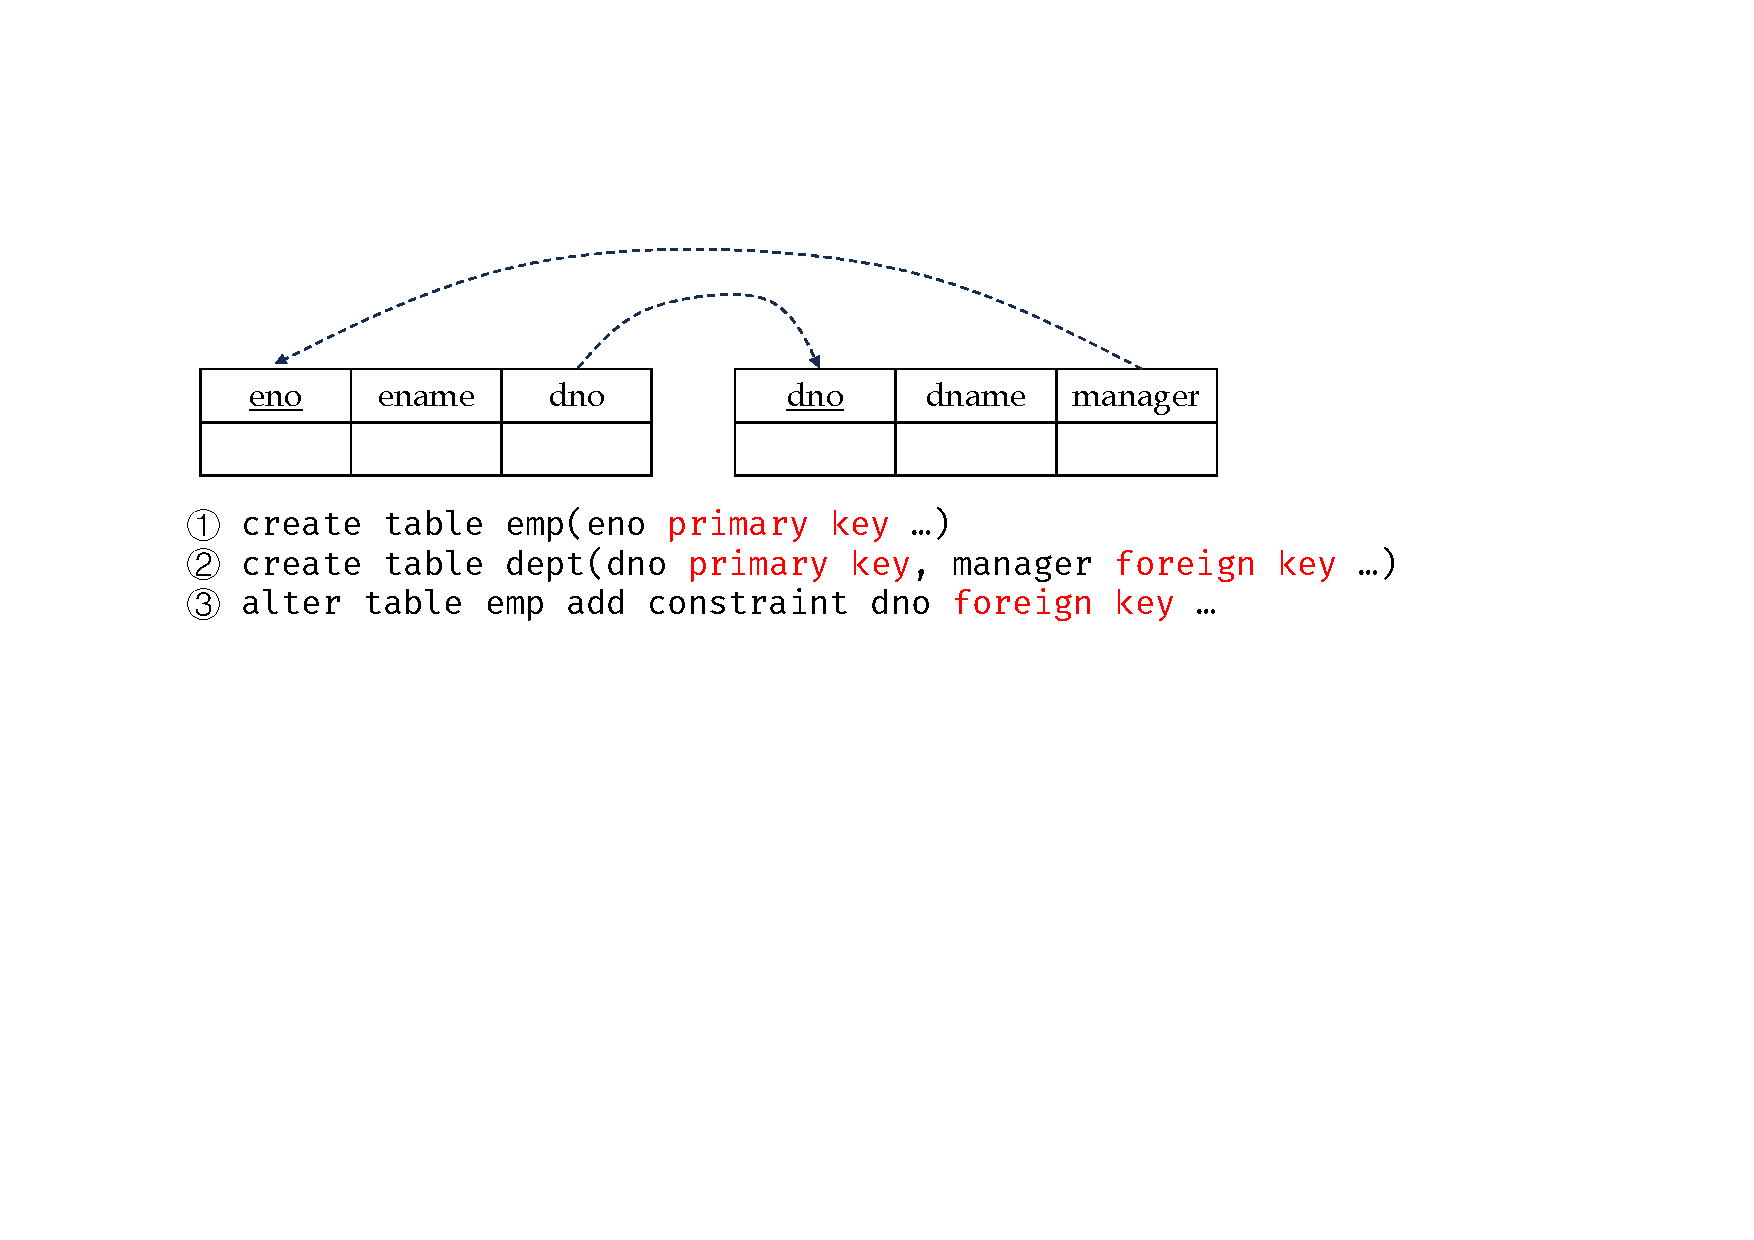
\includegraphics[width=.7\textwidth]{figure/相互参照.pdf}
    \caption{定义两个相互参照的表}
\end{figure}

外键有三种定义方式, 他们的删除时的行为也不一样:
\begin{figure}[H]
    \centering
    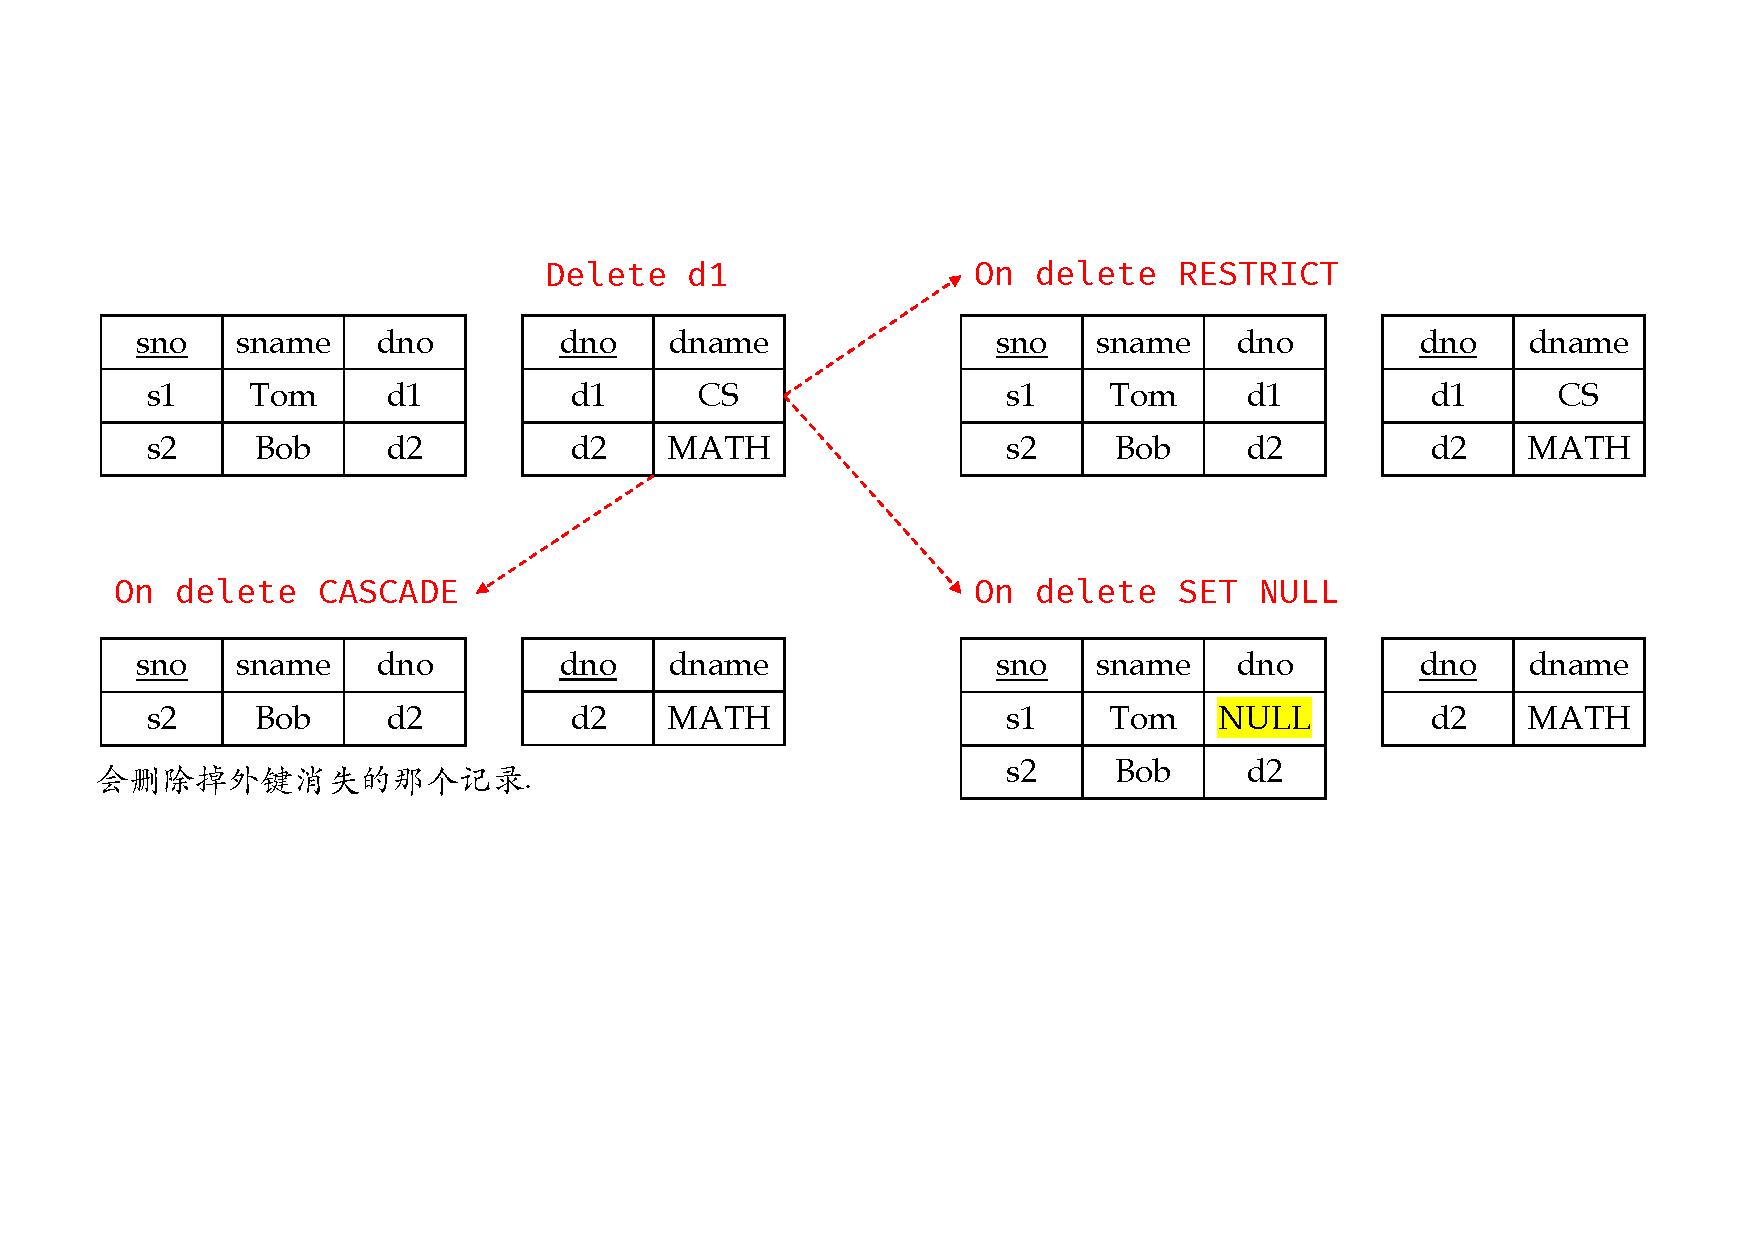
\includegraphics[width=.8\textwidth]{figure/外键删除.pdf}
    \caption{外键的三种定义}
\end{figure}

\begin{lstlisting}[language=SQL]
create table SC (
    sno char(8),
    cno char(10),
    grade smallint,
    primay key (sno, cno),
    check(sno in (select sno from student)),
    check(cno in (select cno from course)))
-- 这里的 check 定义丝毫不等于外码约束
-- 因为 check 定义只有在 SC 表更新才会触发
-- student 中的删除不会触发 check
\end{lstlisting}


相互参照的表 和 自参照的表 插入数据:
\begin{itemize}
    \item 将多个更新操作语句放入一个事务, 在提交时才检查约束.
    \item 使用\textit{延迟约束}.
\end{itemize}

使用延迟约束:
\begin{lstlisting}[language=SQL]
CREATE TABLE Orders (
    OrderID NUMBER GENERATED BY DEFAULT AS IDENTITY PRIMARY KEY,
    CustomerID NUMBER,
    OrderDate DATE,
    CONSTRAINT fk_customer
        FOREIGN KEY (CustomerID)
        REFERENCES Customers(CustomerID)
        DEFERRABLE INITIALLY DEFERRED
);

BEGIN
    INSERT INTO Orders (CustomerID, OrderDate) VALUES (999, TO_DATE('2023-01-01', 'YYYY-MM-DD'));
    -- 其他操作...
    COMMIT; -- 提交时检查约束
END;

SET CONSTRAINT fk_customer DEFERRED;
\end{lstlisting}

SQL Server可以添加一个未验证的约束:
\begin{lstlisting}[language=SQL]
alter table t1 with nocheck add constraint skip_check check (col_a > 1)

alter table t1 nocheck constraint skip_check
insert into t1 values (-2)
alter table t1 check constraint skip_check
\end{lstlisting}

\section{数据库安全性}


\begin{definition}[主体(Principal)]
    主体(principal)是可以授予权限以访问特定数据库对象的对象, 包括登录用户、角色、应用程序.
\end{definition}

MySQL中创建一个主体:
\begin{lstlisting}[language=SQL]
CREATE USER 'username'@'host' IDENTIFIED BY 'password';
GRANT ALL PRIVILEGES ON database_name.* TO 'username'@'host';
\end{lstlisting}

\begin{definition}[客体(Securable)]
    客体(Securable)是指数据库系统中任何可以设置权限的对象. 
    这些对象包括但不限于数据库本身、表、视图、存储过程、函数、列、序列、模式等.
\end{definition}

\begin{figure}[H]
    \centering
    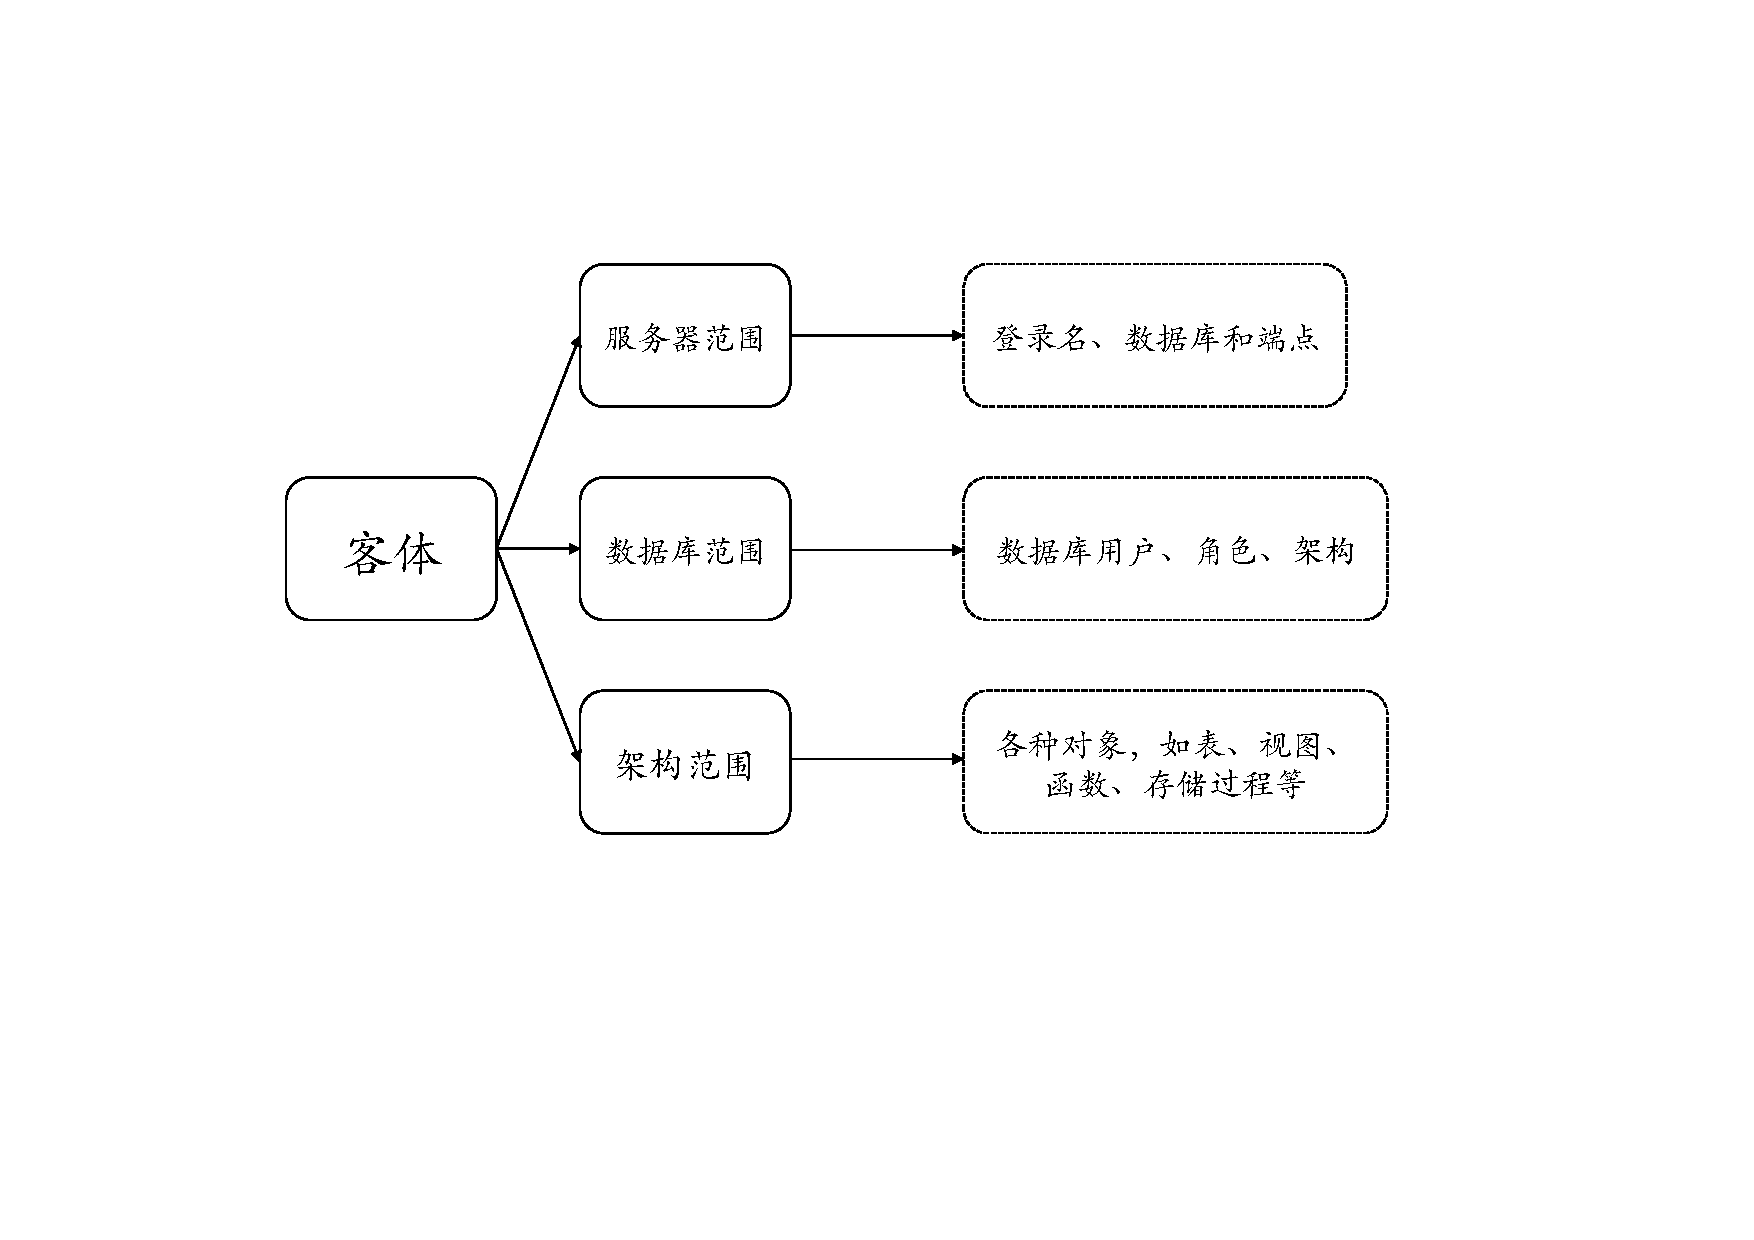
\includegraphics[width=.7\textwidth]{figure/客体.pdf}
    \caption{客体分类}
\end{figure}

\begin{definition}[权限(Permission)]
    权限(Permission)允许主体在安全对象上执行操作.
\end{definition}

\begin{definition}[权限的转授和回收]
    权限的转授和回收: 允许用户把已获得的权限转授给
其他用户, 或者把已授给其他用户的权限再回收上来.
\end{definition}

\begin{definition}[权限图]
    结点是用户, 根结点是DBA.
    \begin{itemize}
        \item 有向边$U_i\to U_j$, 表示用户$U_i$把某权限授给用户$U_j$;
        \item 一个用户拥有权限的充分必要条件是在权限图中有一条从根结点到该用户结点的路径.
    \end{itemize}
\end{definition}

在权限图上回收权限时, 要注意始终保证授权路径起点是DBA。

授权命令:
\begin{lstlisting}[language=SQL]
grant 权限
on    对象名
to    {用户 ... | public}
      [with grant option]
\end{lstlisting}

表级权限: select, update, insert, delete, index, alter, drop, resource等以及它们的总和all

回收权限:
\begin{lstlisting}[language=SQL]
revoke 权限
on 对象
from {用户 [, 用户] ... | public}
\end{lstlisting}

收回权限时, 若该用户已将权限转授给其它用户, 则也一并收回.

\begin{lstlisting}[language=SQL]
grant select, insert on S to Liming with grant option
revoke insert on S from Liming
\end{lstlisting}

\begin{definition}[角色]
    角色是一组相关权限的结合, 即将多个
不同的权限集合在一起就形成了角色.
\end{definition}

创建数据库角色: \verb|create role role_name|.

\begin{figure}[H]
    \centering
    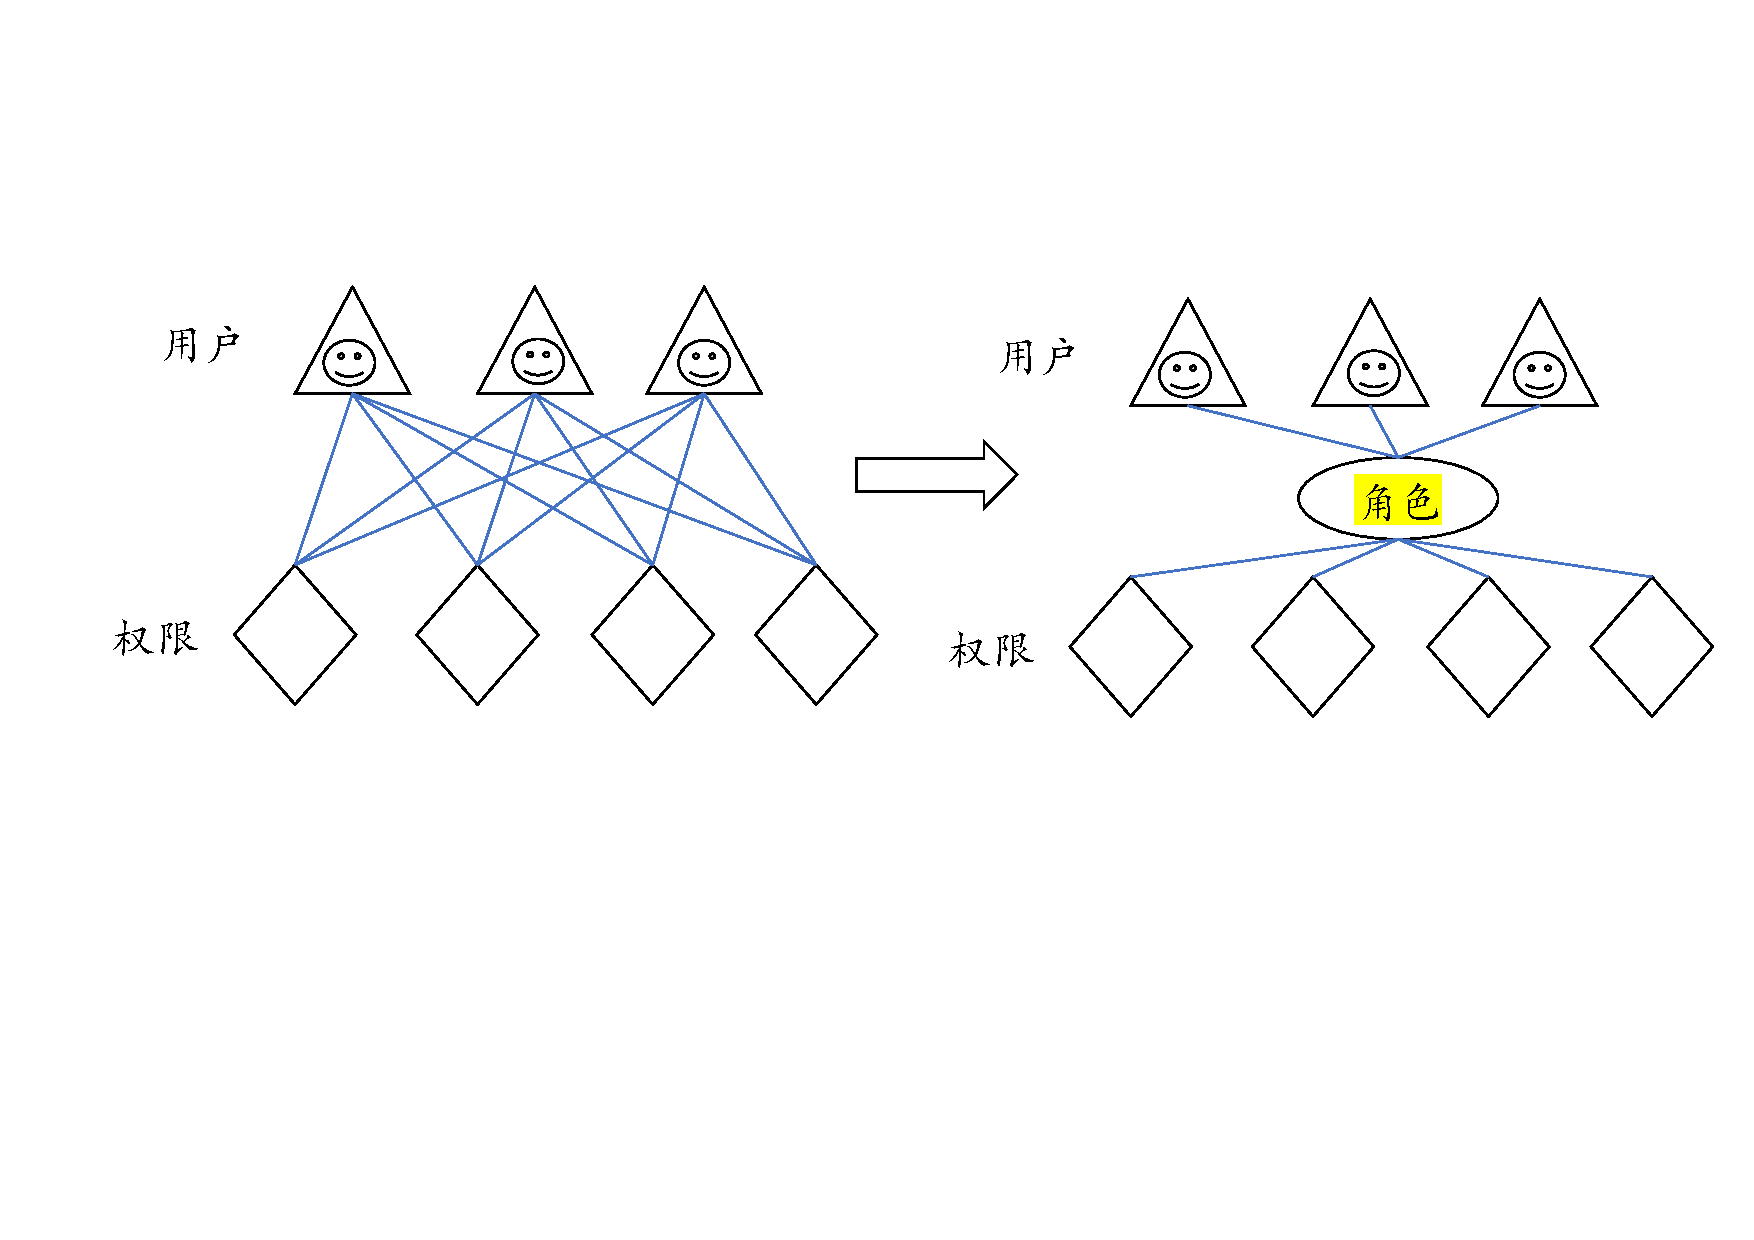
\includegraphics[width=.8\textwidth]{figure/角色.pdf}
    \caption{数据库角色}
\end{figure}

授权Tom只有察看职工平均工资的权限:
\begin{lstlisting}[language=SQL]
create view avg_sal
as
(select avg(sal)
from teacher)

grant SELECT on avg_sal to 'Tom'
\end{lstlisting}

\begin{lstlisting}[language=SQL, caption={普通员工只能查看自己的记录}]
declare @usr char(30)
set @usr = user
select 'The current user is: '+ @usr

select *
from student
where sname = user
\end{lstlisting}

\textbf{访问控制类型}:
\begin{itemize}
    \item 自主访问控制(DAC): 对客体拥有控制权的主体能够将对该客体的访问权自主地授予其它主体, 并在随后任何时刻将这些权限回收;
    \item 强制访问控制(MAC):
    \begin{itemize}
        \item 敏感度标记: 绝密、机密、可信、公开.
        \item 主体: 许可证级别; 客体: 密级.
        \item 保密性规则: 
        \begin{itemize}
            \item 下读: 仅当主体许可证级别高于或等于客体密级时才能读取相应客体
            \item 上写: 仅当主体许可证级别低于或等于客体密级时体才能写相应客体
        \end{itemize}
    \end{itemize}
\end{itemize}

\begin{definition}[审计]
审计就是对指定用户在数据库中的操作情况进行监控和记录, 用以审查用户的相关活动.

审计就是监视和收集指定数据库的活动数据.
\end{definition}

\begin{lstlisting}[language=SQL]
create server audit MyServerAudit to file ...
create server audit specification MyServerAuditSpe
    for server audit MyServerAudit
alter server audit specification MyServerAuditSpe
    add (SERVER_PRINCIPAL_CHANGE_GROUP)
create database audit specification MyDBAudit
    for server audit MyServerAudit
alter database audit specification MyDBAudit
    add ( SELECT ON student )

select event_time, succeeded, statement
from sys.fn_get_audit_file(...)
\end{lstlisting}

\textbf{加密}:
\begin{itemize}
    \item 短语加密: \verb|encryptByPassPhrase|、\verb|decryptByPassPhrase|.
    \item 非对称密钥加密:
\begin{lstlisting}[language=SQL]
create asymmetric key myAsym_key
insert into emp(ename, salary) values ('tom',
    EncryptByAsymkey(Asymkey_ID('myAsym_key'), 100000000))
select DecryptByAsymkey( Asymkey_ID('myAsym_key'), salary)
from emp
where name = 'tom'
\end{lstlisting}
    \item 对称密钥加密.
\end{itemize}

\textbf{SQL注入}:
\begin{itemize}
    \item 认证过程发出的查询语句:
\begin{lstlisting}[language=SQL]
select * from users
where   username = 'jake'
    and PASSWORD = 'jakespasswd'
\end{lstlisting}
    \item 攻击者篡改这个语句:
\begin{lstlisting}[language=SQL]
select * from users
where   username = 'jake'
    and PASSWORD = 'jakespasswd' or 'x' = 'x'
\end{lstlisting}
\end{itemize}

\textbf{统计数据库安全性}:

在某些高敏感性场景下, 为了保护隐私, 系统会限制用户只能进行 聚集查询(Aggregate Queries).
攻击者仍可能通过多次合法的聚集查询 推理出某个个体的具体值, 这就叫作“统计推断攻击(Statistical Inference Attack)”.
\begin{itemize}
    \item 漏洞一: 个体太少. 如果只有一两个学生选了这门课, 那平均值就几乎等于个体值, 容易被推测出来.
    \item 漏洞二: 多次查询, 太多交叠. 通过多个查询结果相减来推出个体值.
\end{itemize}

我们加入防范措施:
\begin{itemize}
    \item 查询引用的数据不能少于 $n$ 条元组;
    \item 任意两个查询的交集不能超过 $m$ 条元组;
    \item 那么在上面两条的保证下, 推出个体信息至少需要 $1 + (n-2)/m$ 次查询.
\end{itemize}

连接推理: 可以通过两张表里相同列的连接, 推理出个人信息.

$k$-anonymity:
\begin{definition}[准标识符(Quasi-Identifier, QI)]
    准标识符: 指一组属性(如年龄、性别、邮编), 
    单独使用时无法直接标识个体, 但结合外部数据(如选民名单)可能定位到具体个人.
\end{definition}

\begin{definition}[泛化]
将具体值替换为更宽泛的范畴(如年龄“25岁” → “20-30岁”).
\end{definition}

\begin{definition}[抑制]
    直接删除高风险数据(如罕见疾病患者的邮编).
\end{definition}

使所有记录的准标识符组合形成至少$k$个相同分组.

\begin{definition}[$k$-anonymity]
    若数据满足$k$-anonymity, 则对任意记录$r$, 存在至少$k-1$条记录满足:
    \begin{align*}
        \forall r \in D, |\{r'\in D| \text{QI}(r')=\text{QI}(r)\}| \geq k.
    \end{align*}
\end{definition}
